\section{Introduction}


The landscape of text-to-image (T2I) generation has evolved at breakneck speed, rapidly transitioning from the foundational U-Net~\cite{sd} architectures to the scalable era of Diffusion Transformers~\cite{DiT}. Recently, this evolution has reached a new pinnacle with the emergence of single-stream diffusion transformers, a unified framework exemplified by state-of-the-art models like Z-Image~\cite{zimage} and HunyuanImage-3.0~\cite{hunyuanimage3}. Unlike traditional dual-stream models (\textit{e.g.,} Flux~\cite{flux1kontext}) that process text and pixels separately, this new paradigm fundamentally treats visual and textual data as a single, unified sequence handled by a monolithic transformer backbone~\cite{zimage}. The efficiency of this architectural grand unification is remarkable: Z-Image Turbo, for instance, generates stunningly photorealistic imagery with only 6B parameters, signaling that the recently emerging pure single-stream framework is not merely an architectural variant, but the blueprint shaping the next generation of foundational models.


\begin{figure}[t]
	\centering
	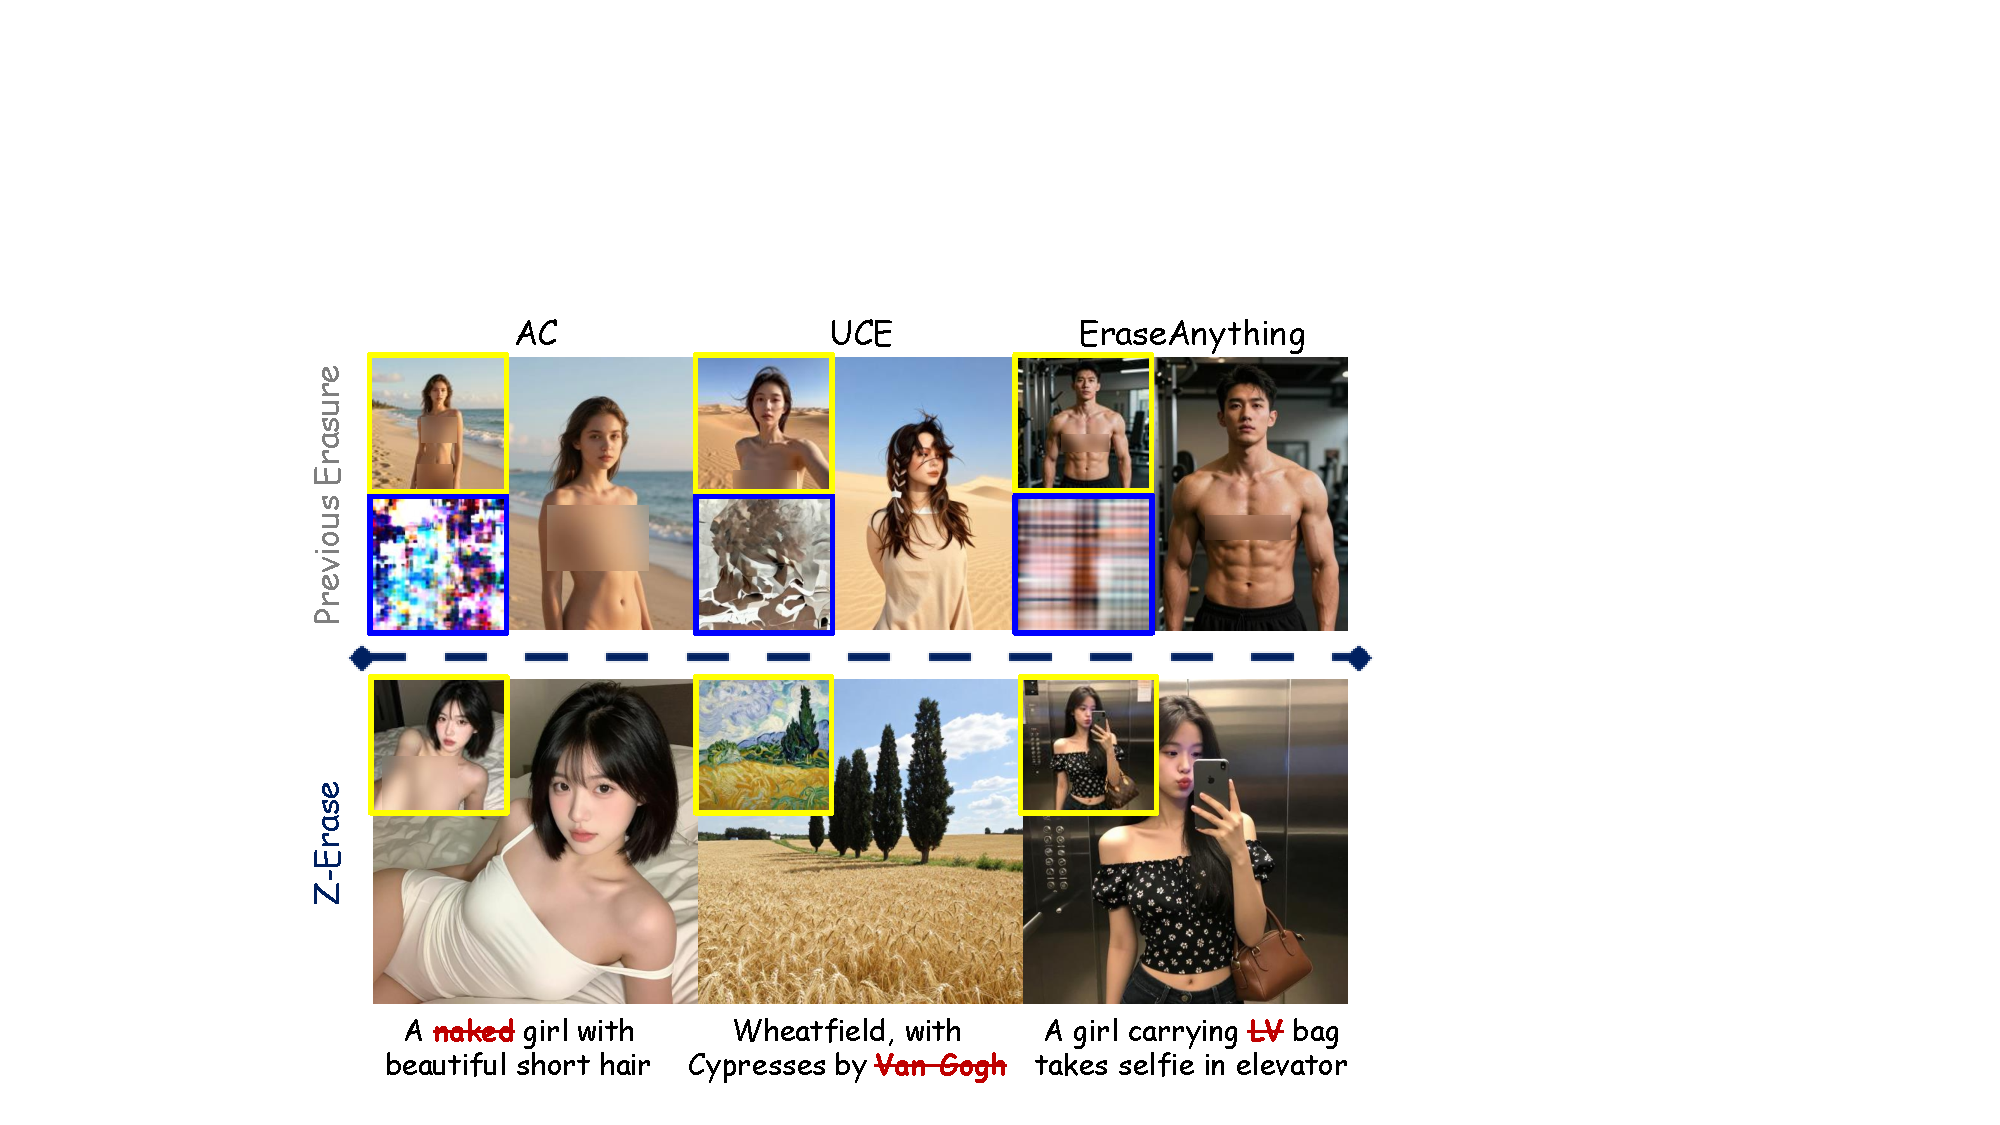
\includegraphics[width=0.9\linewidth]{fig/teaser.pdf}
    \caption{We introduce \textbf{Z-Erase}, a concept erasure method tailored for single-stream models. \textit{First row}: Prior methods adapted via our \emph{Stream Disentangled Concept Erasure Framework} are tested with the ``nudity" concept, showing under-erasure (AC, EraseAnything) or severe artifacts (UCE). \textcolor{blue}{Blue} boxes reveal the generation collapse caused by naive fine-tuning without our adaptation. \textit{Second row}: Z-Erase effectively removes target concepts while preserving quality. Original outputs are in \textcolor{darkyellow}{yellow} boxes. Sensitive content pixelated.}
    \label{fig:teaser}
    \vspace{-13pt}
\end{figure}



However, this generative prowess comes with significant risks. If the training data is not carefully filtered, foundational models can effortlessly absorb and reproduce copyrighted entities, Not-Safe-For-Work (NSFW) material, and biased imagery~\cite{barez2025openproblemsmachineunlearning}. As these models gain broader adoption, the societal risks of such unrestricted generation become acute. In response, concept erasure has emerged as a vital safety alignment strategy~\cite{ca, esd}. Instead of re-training the entire model, concept erasure selectively removes undesired target concepts while maintaining the model's utility and performance on normal content.


While concept erasure is well-established for Stable Diffusion (SD)~\cite{sd} and Flux~\cite{flux1kontext} series, we find that directly transferring these methods to pure single-stream models leads to \emph{consistent generation collapse}, as shown in Fig.~\ref{fig:teaser} (\textcolor{blue}{blue} boxes). Through careful analysis, we trace the failure to the unified single-stream architecture, as detailed in Section~\ref{sec:motivation}. Unlike previous models that isolate text-image interactions within separate modules, single-stream transformers fuse both modalities into a unified self-attention mechanism with shared weights~\cite{zimage}. Consequently, optimizing shared parameters to suppress text concepts will inevitably damage visual backbone's synthesis capability, leading to catastrophic noise outputs.



To tackle this issue, we introduce \textbf{Z-Erase}, a concept erasure method tailored for single-stream models. First, to enable existing erasure methods on single-stream models, we propose \textbf{Stream Disentangled Concept Erasure Framework}, a structural intervention that decouples parameter updates in single-stream models. By freezing the visual processing pathway while allowing low-rank adaptations (LoRAs)~\cite{lora} only on textual hidden states, we create a safe optimization subspace that protects the image generation backbone. Within this subspace, prior erasure methods can operate on single-stream models.

However, even with this structural fix, we find that the unified attention space of single-stream models remains highly sensitive, making it difficult to balance erasure of target concept against preservation of unrelated content, as shown in Fig.~\ref{fig:teaser} (first row). To address this, we further introduce a \textbf{Lagrangian-Guided Adaptive Erasure Modulation} algorithm, which solves this trade-off as a constrained optimization problem by dynamically maximizing erasure only when the preservation loss remains within a strict tolerance. In addition to the algorithm design, we also provide a rigorous theoretical analysis proving that our algorithm can converge to a Pareto stationary point~\cite{yu2020gradientsurgerymultitasklearning}. Experiments demonstrate that Z-Erase successfully solves this optimization dilemma, ensuring robust ethical safety with minimal and controllable degradation in utility.

To the best of our knowledge, Z-Erase is the first effective concept erasure method tailored for the emerging single-stream T2I paradigm. Our main contributions are:
\begin{itemize}[leftmargin=*]
\item \textbf{Single-stream attention localization}. We identify that generation collapse in single-stream models stems from shared projection weights. Beyond this, we further find that attention maps allow precise token-level localization, enabling selective erasure of targeted content.
\item \textbf{Stream disentangled concept erasure framework}. We propose a structural intervention for single-stream models. By injecting learnable adaptations exclusively into textual hidden states while freezing the visual backbone, we construct a safe optimization subspace that enables existing erasure methods to work on single-stream models.
\item \textbf{Lagrangian-Guided Adaptive Erasure Modulation}. To resolve the sensitive trade-off between erasure and preservation, we introduce a dynamic algorithm building upon this framework that maximizes erasure within a strict utility tolerance, and provide a rigorous convergence guarantee to a Pareto stationary point.
\end{itemize}